\documentclass[11pt,a4paper]{article}
\usepackage[ngerman]{babel}
\usepackage{graphicx}
\usepackage{float}
\usepackage[textfont=it, width= 0.75\textwidth, textformat=period, labelformat=empty, justification=RaggedRight, singlelinecheck=false]{caption}
\usepackage[labelformat=empty]{subcaption}
\usepackage{wrapfig}
\usepackage{wallpaper}
\usepackage{booktabs}
\usepackage{amsmath}
\usepackage{esvect}
\usepackage{url}
\usepackage{lmodern}
\usepackage[colorlinks=true,linkcolor=black,urlcolor=cyan,citecolor=black]{hyperref}
\usepackage[left=2.5cm,right=2.5cm,top=2cm,bottom=2cm]{geometry}

%Konfiguration von Absätzen
\setlength{\parindent}{0pt}
\setlength{\parskip}{5pt}

\begin{document}
\thispagestyle{empty}

{\scshape\large\centering Gymnasium Eversten Oldenburg \\}
\vspace{-10pt}
\noindent\rule{\textwidth}{0.5pt} %Horizontale Linie
\vspace{5pt}
{\large\bfseries\centering Aerodynamik von Modellraketen: Luftwiderstand und Flugstabilität \\}
{\centering\itshape Jeremias Beth und Benjamin Lips \\}

\vspace{-5pt}
\subsection*{Zielsetzung}
\vspace{-10pt}

In dieser Arbeit wird der Einfluss der Raketenspitze auf den Flug einer Modellrakete untersucht. Diese Untersuchung findet anhand der selbst gebauten Rakete FTV statt, wobei Luftwiderstand und Flugstabilität untersucht wurden. Es wurden fünf Formen von Raketenspitzen betrachtet.


\vspace{-5pt}
\subsection*{Luftwiderstand}
\vspace{-10pt}

Die Untersuchung des Luftwiderstandes hat das Ziel, von den Spitzen die mit der grö"sten Flughöhe zu ermitteln. Dafür wird im Windkanal der Widerstandsbeiwert von FTV mit jeder der Spitzen bestimmt. Anschlie"send wird ein möglichst simples Modell entwickelt, mit dem die Flughöhe bestimmt wird. 

\begin{figure}[H]
	\begin{subfigure}[l]{0.49\textwidth}
		\centering
		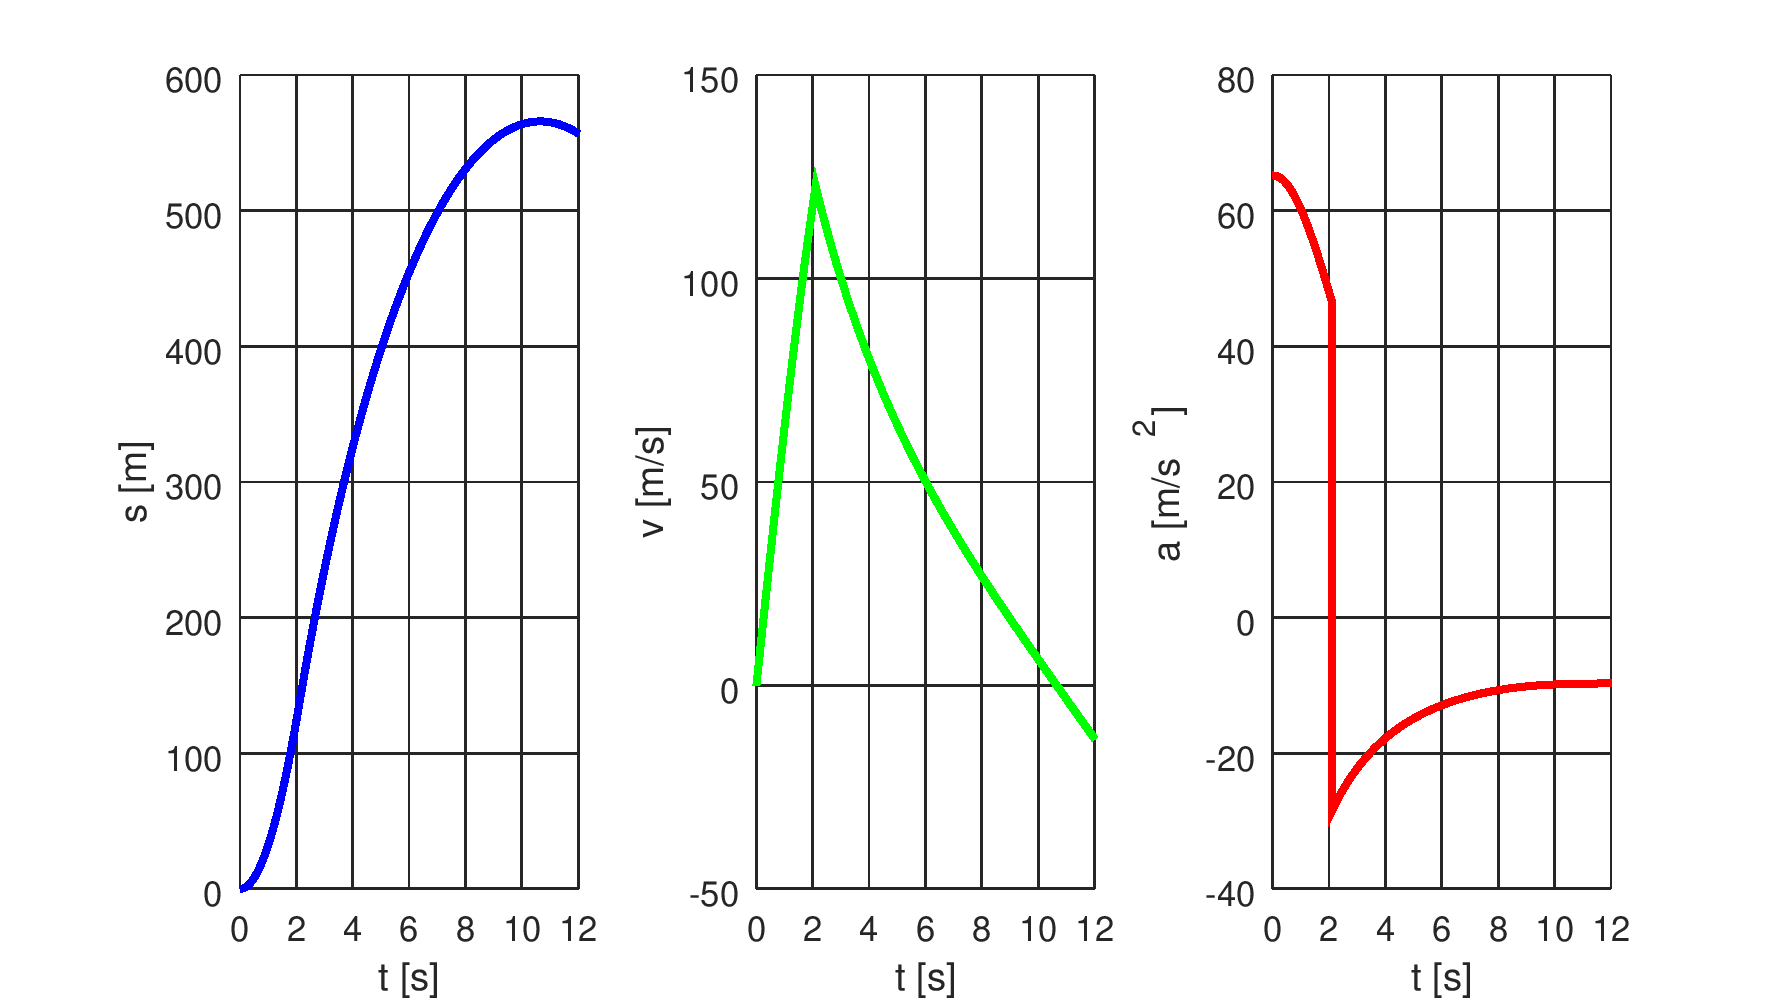
\includegraphics[width=\textwidth]{Bilder/Flugsimulation.png}
		\caption{Flugsimulation von FTV mit ogiver Spitze}
		\label{sfig-Flugsimulation}
	\end{subfigure}
	\begin{subfigure}[r]{0.49\textwidth}
		\centering
		\includegraphics[width=\textwidth]{Bilder/Simulierte-Flughöhe.png}
		\caption{In der Simulation erreichte Flughöhe}
		\label{sfig-Simulierte-Flughöhe}
	\end{subfigure}
\end{figure}

\vspace{-10pt}
\begin{wrapfigure}{r}{0.3\textwidth}
	\vspace{-11pt}
	\centering
	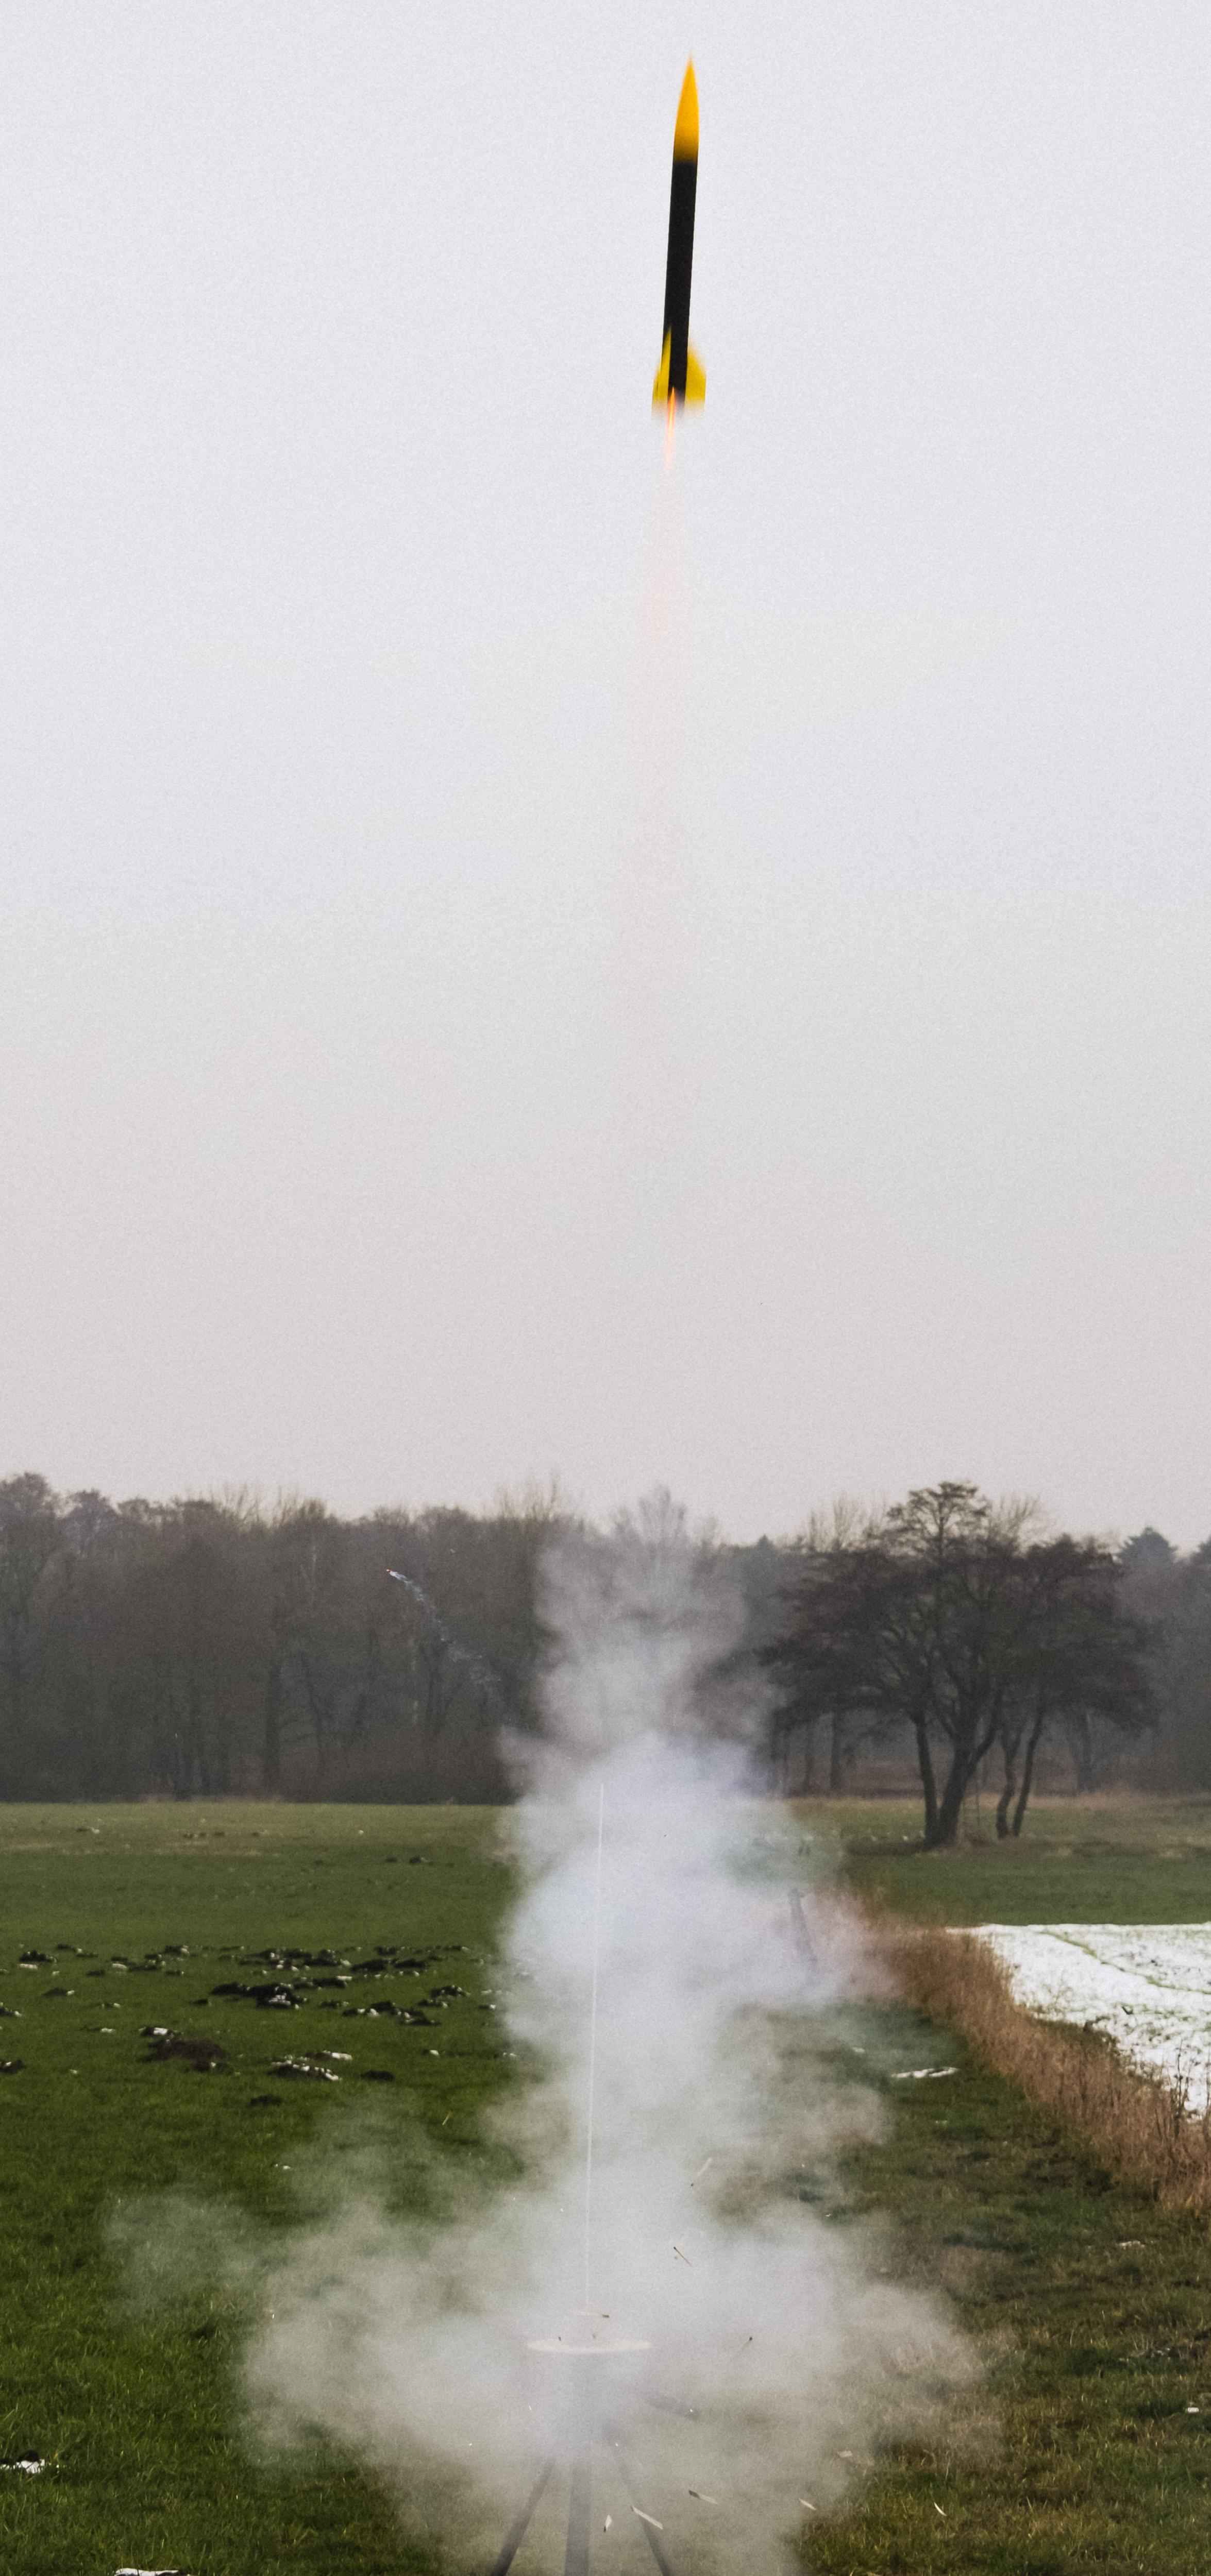
\includegraphics[width=0.3\textwidth]{Bilder/Flugversuch-Start.jpg}
	\caption{Start von FTV}
\end{wrapfigure}

Der Versuch ergab, dass die Ogive als Spitzenform im Unterschallbereich den anderen betrachteten Formen in der erreichten theoretischen Flughöhe überlegen war. Die Hypothese, dass ein knickfreier Übergang zwischen Körperrohr und Spitze die Flughöhe verbessert, wurde bestätigt. Die Haack Spitze zeigte allerdings entgegen der Erwartung keine Vorteile.  


\vspace{-5pt}
\subsection*{Flugstabilität}
\vspace{-10pt}

Die Untersuchung der Flugstabilität fand zunächst theoretisch statt, wobei ein Verfahren zur Berechnung des Druckpunktes eingesetzt wurde. Zusätzlich wurde ein Versuch im Windkanal durchgeführt.
Die theoretische Untersuchung ergab, dass FTV mit allen Spitzen ausreichende Flugstabilität aufweist. Diese Ergebnisse konnten durch den Versuch im Windkanal bestätigt werden, wobei zusätzlich festgestellt wurde, dass sich die Rakete quer zum Wind stabil ausrichten kann. Das ist jedoch im Flug sehr unwahrscheinlich.

Im Vergleich der Spitzen lässt sich keine als optimal feststellen. Welche Spitze für eine konkrete Rakete in Bezug auf die Flugstabilität am besten ist, hängt davon ab, ob eine zu gro"se oder kleine Kaliberzahl vorliegt.


\vspace{-5pt}
\subsection*{Weitere Informationen}
\vspace{-10pt}

Das Vollständige Projekt ist verfügbar unter: \\
\url{https://github.com/FTVLab/Aerodynamik-von-Modellraketen}


\end{document}